\documentclass[svgnames]{article}
\usepackage[a4paper,margin=30mm]{geometry}
\usepackage{xspace}
\usepackage{stix}
\usepackage{enumitem}

\setlist[description]{font=\sffamily\bfseries\color{DodgerBlue},labelwidth=\textwidth}
\usepackage{graphicx}
\synctex=1

\usepackage{cmap} % fix search and cut-and-paste in Acrobat
\usepackage[T1]{fontenc}
\usepackage[utf8]{inputenc}
\setcounter{secnumdepth}{0}

\usepackage{listings}\lstset{language=[LaTeX]TeX,framerule=2pt}
\lstset{language=[LaTeX]TeX,
        texcsstyle=*\bfseries\color{Blue},
        backgroundcolor=\color{Ivory},
        numbers=none,
        breaklines=true,
        keywordstyle=\color{Blue},
        commentstyle=\color{Brown},
        tabsize=2,
        morekeywords={UnitCode,UnitName,UnitURL,QuizzesURL,BreadCrumb,University,Department,quiz,quizlist,discussion,
                      question,choice,Choice,response,correct,incorrect,whenRight,whenWrong,answer},
        resetmargins=true,
}
% hyperref links to ctan
\newcommand\ctan[1]{\href{https://www.ctan.org/pkg/#1}{\texttt{#1}}}

\usepackage{xparse}
\NewDocumentCommand{\Verb}{v}{{\color{blue}#1}}

\newcommand\Section[1]{\subsection{\textcolor{blue}{#1}}}

\makeatletter
\author{Andrew Mathas}
\usepackage{tikz}
\usetikzlibrary{shadows.blur}
\tikzset{shadowed/.style={blur shadow={shadow blur steps=5},
                          bottom color=LightSkyBlue!30,
                          draw=MidnightBlue!70,shade,
                          font=\normalfont\Huge\bfseries\scshape,
                          rounded corners=8pt,
                          top color=SkyBlue,
      },
      boxes/.style={draw=MidnightBlue,
                    fill=Cornsilk,
                    font=\sffamily\small,
                    inner sep=5pt,
                    rectangle,
                    rounded corners=8pt,
                    text=RoyalBlue,
     }
}
\def\mathquiz@version{Version 5.0}
\def\MathQuiz{\textcolor{blue}{\textsc{MathQuiz}}\xspace}
\def\MathQuizTitle{
  \begin{tikzpicture}[remember picture,overlay]
      \node[yshift=-3cm] at (current page.north west)
        {\begin{tikzpicture}[remember picture, overlay]
          \draw[shadowed](30mm,0) rectangle node[white]{MathQuiz} (\paperwidth-30mm,16mm);
          \node[MidnightBlue,font=\normalfont\small\itshape] at (\paperwidth/2,2mm) {\small On-line quizzes written in LaTeX};
          \node[anchor=west,boxes] at (4cm,0cm) {\@author};
          \node[anchor=east,boxes] at (\paperwidth-4cm,0) {\mathquiz@version};
         \end{tikzpicture}
        };
   \end{tikzpicture}
   \vspace*{20mm}
}


\def\@oddfoot{\MathQuiz -- \mathquiz@version\hfill\thepage}

\usepackage[colorlinks=true,linkcolor=blue,urlcolor=blue]{hyperref}
\hypersetup{pdfcreator={ Generated by pdfLaTeX },
            pdfinfo={Author  ={ Andrew Mathas },
                     Keywords={ web quizzes, latex, tex4ht, make4ht, python, mathematics},
                     License ={ LaTeX Project Public License v1.3c or later },
                     Subject ={ Write on-line quizzes using LaTeX (and TeX4ht) },
                     Title   ={ smartunits - \mathquiz@version }
            },
}
\makeatother

\begin{document}

    \MathQuizTitle

    \tableofcontents

    \MathQuiz is a system for writing on-line quizzes using \LaTeX.
    Professional mathematicians and educators use \LaTeX\ to write their
    research papers, books and teaching materials. \MathQuiz provides an
    easy way for anyone who knows \LaTeX\ to create an on-line quiz from
    a `normal'' \LaTeX file. The allows the quiz author to concentrate
    on the content of quizzes unencumbered by the technicalities of HTML
    and javascript, which they will never need to know.

    The on-line quizzes constructed by \MathQuiz follow a particular format and
    layout, although this has been designed to be easy to customise.
    Currently \MathQuiz supports the following types of questions:
    \begin{itemize}[nosep]
      \item Multiple choice questions with a unique correct answer
      \item Multiple choice questions zero or more correct answers
      \item Questions with numerical answers
    \end{itemize}
    Each time a student answers a questiuon they are told whether they
    are right or wrong and it is possible for the quiz author to give
    targeted feedback ti the student based on their answer. In
    principle, anything that can be written using \LaTeX\ can appear in
    the on-line quiz. In practise, the \LaTeX\ is converted to HTML using
    \href{https://www.tug.org/applications/tex4ht/mn.html}{\TeX 4ht}, and
    \href{https://github.com/michal-h21/make4ht}{make4ht}, so you can
    use anything in \LaTeX\ that is understood by these packages, which is almost
    everything.

    The easiest way to explain how \MathQuiz works is by example, so
    consider the following \LaTeX\ file.

    \lstinputlisting{example.tex}

    This defines quiz with one multiple choice question, and four
    possible responsible responses: $1$, $2$, $3$ and~$4$. The first
    answer, $1$, is correct and the remaining answers are wrong. If the
    person selects a given answer then they will be told whether or not
    their answer is correct and the corresponding \verb!\response!
    message will be printed. For example, in the quiz produced by
    \MathQuiz if you select option (c) then you will see something like
    this:

    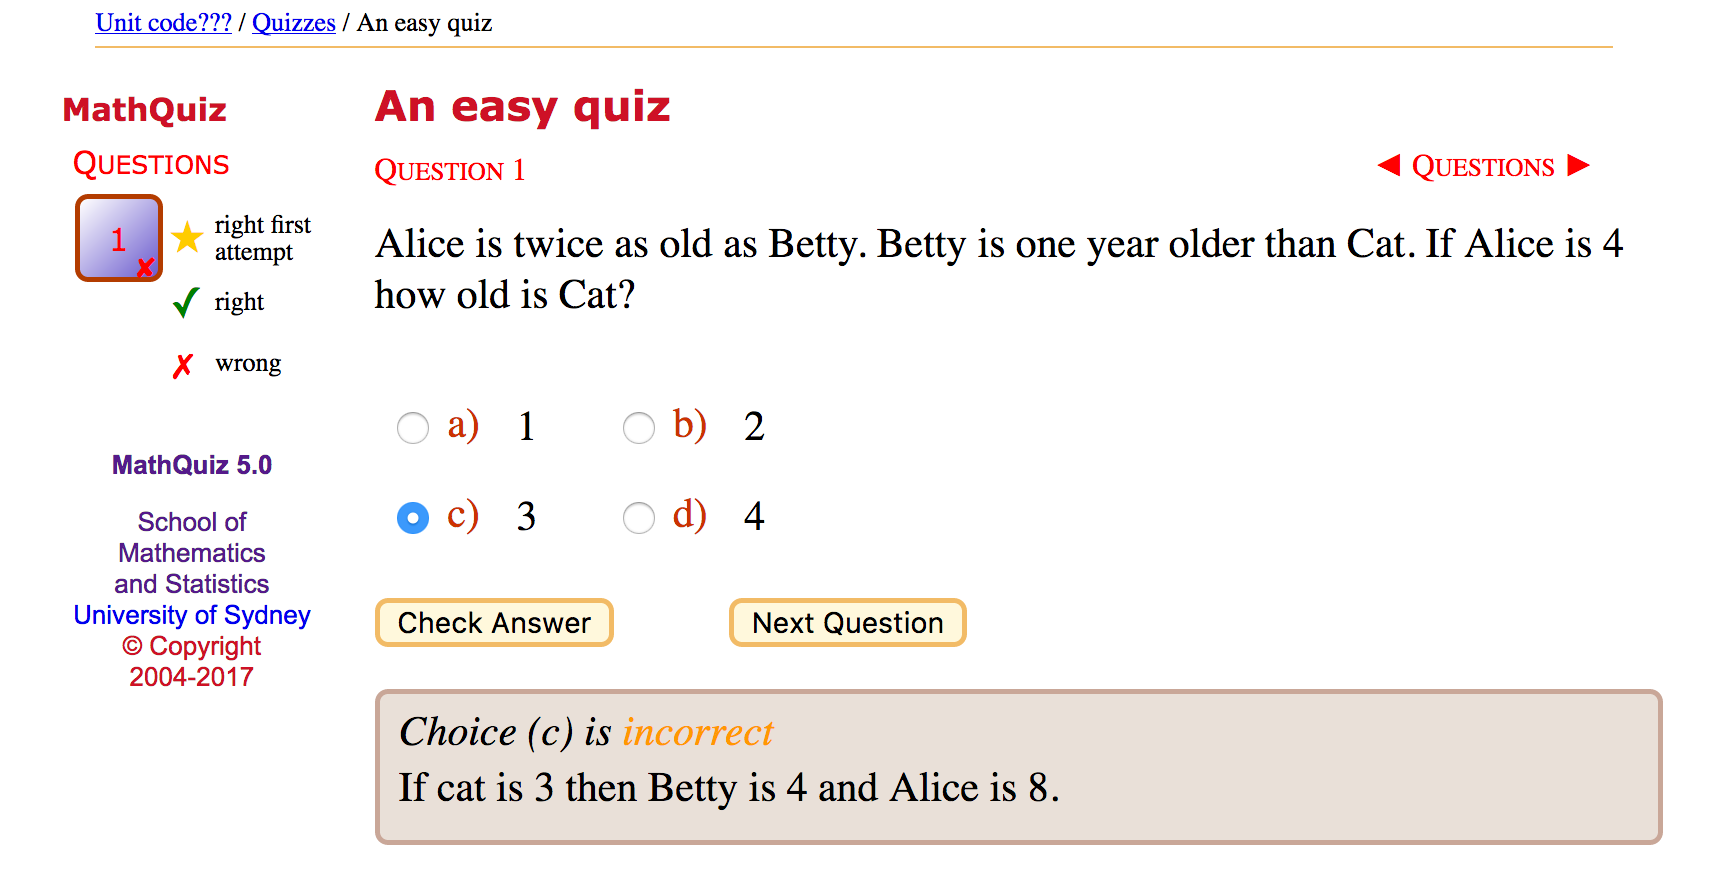
\includegraphics[width=\textwidth]{easy_quiz-html}

    As this is a \LaTeX\ file you can run this through (pdf)latex to
    produce a pdf file (or a dvi or postscript etc), which produces
    the output:

    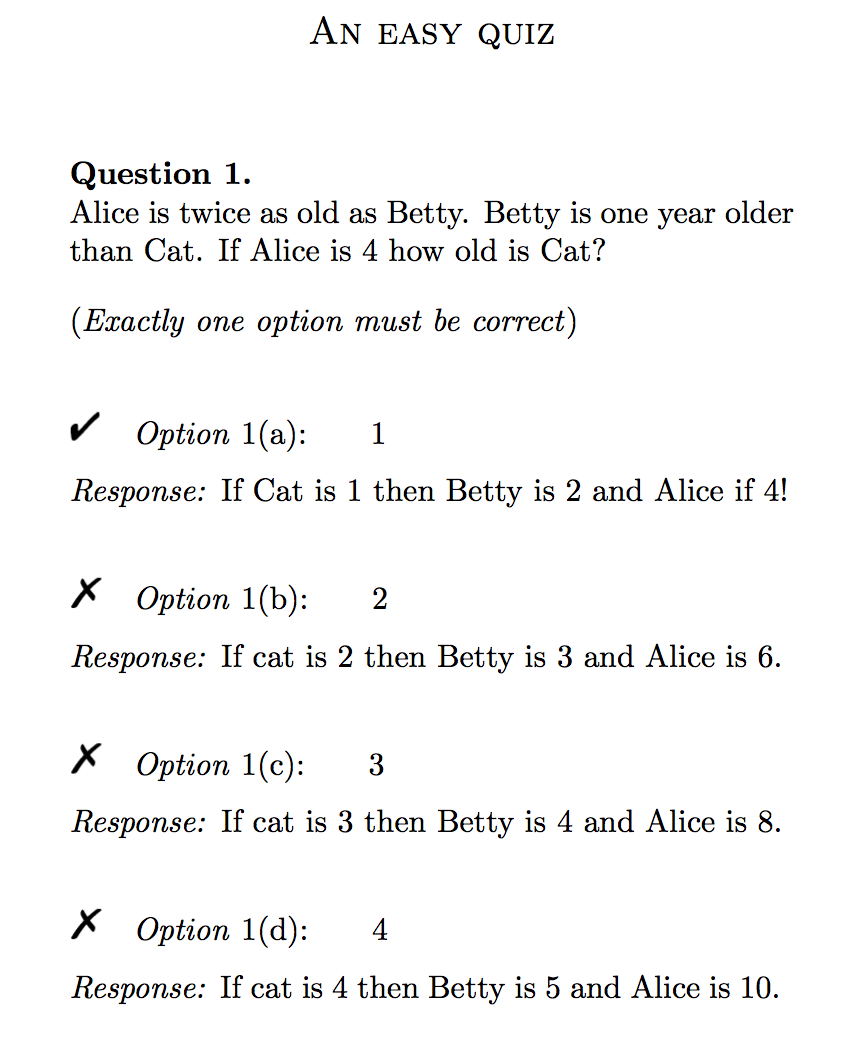
\includegraphics[width=0.5\textwidth]{easy_quiz}

    \Section{The \MathQuiz document class}
    \Section{System requirements, installation and configuration}

    To use the system you will need to have all of the following programs installed:
    \begin{itemize}
         \item \LaTeX, \TeX 4ht and \textsc{make4ht}
         All of these are available through standard \TeX\ installations
         such as \TeX live
         \item Python3
         \item \MathQuiz
    \end{itemize}

    \MathQuiz will soon be submitted to ctan, in which case it will soon
    be incorporated into \TeX live.

    \Section{Authors}

\MathQuiz is based on an initial prototype that was written by Don Taylor in
2001. Since 2004 the program has been maintained and developed by Andrew
Mathas. Some of the initial code remains but quite a

\Section{Licence}

Copyright (C) 2013-2017

GNU General Public License, Version 3, 29 June 2007

This program is free software: you can redistribute it and/or modify it under
the terms of the GNU General Public License (GPL) as published by the Free
Software Foundation, either version 3 of the License, or (at your option) any
later version.

This program is distributed in the hope that it will be useful, but WITHOUT ANY
WARRANTY; without even the implied warranty of MERCHANTABILITY or FITNESS FOR A
PARTICULAR PURPOSE.  See the GNU General Public License for more details.



MathQuiz:
======================================

MathQuiz is a system for writing interactive web based quizzes, particularly
those that involve mathematics. The quizzes are first written in LaTeX and
then converted into HTML files using MathQuiz, which is written in python. The
conversion from LaTeX to HTML is done behind the scenes using TeX4ht.

Once the system is installed, MathQuiz is used directly from the
command line. For example, if quiz1.tex is a latex file for a quiz then:
    * latex quiz1         produces a "readable" dvi file for the quiz
    * pdflatex quiz1      produces a "readable" pdf file for the quiz
    * mathquiz quiz1      creates the web page quiz1.html


Installation
------------

MathQuiz has several different components which need to be installed into quite
different places. First, decide where you want to put the source files for MathQuiz.
This will either be in somewhere in your home directory, or something like
/usr/local/src if you want to install the system for general use. This directory
should NOT be accessible from your web server.

Change to this directory and unpack the tar file mathquiz.tgz using
    tar zxf mathquiz.tgz
This will create a directory called mathquiz in your current directory which contains
the files:
    README    -  this file
    latex/    -  the latex class file for running mathquiz
    mathquiz  -  the shell script that runs mathquiz
    src/      -  contains the python scripts for writing the web pages
    web/      -  contains the java script, css and image files needed by MathQuiz

To complete the installation of MathQuiz on your system you need to:
    1. Copy, or move, the directory into the directories used by your web server. This
       can either be in your own directories or in the "system" web directories. For this
       you would do something like
           cp -R web /<path to top of web server>/MathQuiz
       In particular, I recommend renaming this directory MathQuiz when you copy it and
       not calling it web!

    2. Copy, or move, the file latex/mathquiz.cls into the directories searched by latex.
       Again this can be in your own directories (in Unix you can tell tex which
       directories to search using the TEXINPUTS environment variable. If mathquiz.cls is
       installed in a system directory then everyone will be able to use MathQuiz.

    3. Edit the script mathquiz. At the top of the script you will find two variables:
        o MathQuizSRC = directory where you unpacked mathquiz.tgz
        o MathQuizURL = relative URL for the MathQuiz on your web server. This is the
              URL pointing to the files in the directory web/ above. Note that this is a
              relative URL and not the full path to a directory. To access these files
              from your browser you would go to
                http://your.web.server/<MathQuizURL>/

    4. Move the script mathquiz to somewhere in your path like /usr/local/bin.

MathQuiz should now be ready to use. To test it change to the directory on your web
server which contains the files in the directory web/ above. This directory contains
a doc directory and inside this directory you will find the file mathquiz-manual.tex
which is the documentation for using MathQuiz. You should now be able to:
    o latex mathquiz-manual     - produce a dvi version of the manual for printing
    o mathquiz mathquiz-manual  - create the web pages for the online version of the
        manual which you will be able to access by going to
          http://your.web.server/<MathQuizURL>/doc/mathquiz-manual.html

Local configuration
-------------------

The "style" of the online quizzes is controlled by the file src/mathquizLocal.py. If you want to
change this format of the quiz pages then the easiest way to do this is to make a copy of
mathquizLocal.py, say to mathquizMyStyle.py, and then edit this file directly. To see what the
new style looks like you can run the mathquiz script with an optional argument which tells
mathquiz to use your style instead:
    mathquiz -l mathquizMyStyle quizfile.tex
Using mathquiz to regenerate the html files is quite time consuming, so while you are editting this
file you will find it easier if you ask mathquiz not to delete the intermediate files that it
creates each time. To do this first run mathquiz with the -x option and thereafter use -f:
    mathquiz -l mathquizMyStyle -x quizfile.tex   \# tells MathQuiz not to delete intermediate files
    mathquiz -l mathquizMyStyle -f quizfile.tex   \# "fast" option when intermediate files exist
Once the new page format is finalized it can be made the default by setting
    MathQuizOptions="--local=mathquizMyStyle"
at the top of the mathquiz shell script.

The easiest way to change mathquizLocal.py is simply to edit the "decorating" html that this file puts
around the quiz page. You may also need to change the CSS style sheet for mathquiz which is the file
web/mathquiz.css. More sophisticated versions of mathquizLocal.py where you change the underlying
python code are of course possible. For example, at the Unviersity of Sydney our version of this file
calls our content management system directly and uses this to create the web page for the quiz.

    \Section{Command line options}

    The following options can either be used inside \Verb|\MathQuiz| to
    control the formatting \textit{locally} for just the unit being


    \begin{description}
       \item[ -h, --help]            show this help message and exit
       \item[-u MATHQUIZURL, --url MATHQUIZURL]
                    relative URL for MathQuiz web files
       \item[-l LOCAL\_PAGE, --local LOCAL\_PAGE]
                    local python code for generating the quiz web page
       \item[-p, --pst2pdf]
          Use pst2pdf to fix issues with images generated by pstricks
       \item[--initialise]
          initialise files and setings for mathquiz
          \item[--settings]
          list system settings for mathquiz
          \item[--settings-edit]      edit mathquiz settings
          \item[--build MATHQUIZ\_MK4] build file for make4ht
          \item[--mathjax MATHJAX]    URL for mathjax
          \item[-q, --quiet]          suppress tex4ht messages (also -qq etc)
    \end{description}


\begin{verbatim}
.. _`Andrew Mathas`: http://www.maths.usyd.edu.au/u/mathas/
.. _GPL: https://www.gnu.org/licenses/gpl-3.0.en.html
.. _LaTeX: https://www.latex-project.org/
.. _MathQuiz: http://www.maths.usyd.edu.au/u/MOW/MathQuiz/doc/mathquiz-manual.html
.. _Python: https://www.python.org
.. _TeX4ht: http://www.tug.org/tex4ht/
.. _texlive: https://www.tug.org/texlive/
\end{verbatim}

\end{document}
